% ============================================================
%  CXL 调研报告 —— Beamer 演示文稿
%  编译引擎：XeLaTeX（支持中文）
%  编译命令：xelatex cxl_presentation.tex
%  屏幕比例：16:9（宽屏）
% ============================================================

\documentclass[UTF8,9pt,aspectratio=169]{beamer}

% ============================================================
%  中文与字体设置
% ============================================================
\usepackage{xeCJK}
\setCJKmainfont{Songti SC}
\setCJKsansfont{Heiti SC}
\setCJKmonofont{STFangsong}

% ============================================================
%  主题与配色
% ============================================================
\usetheme{Darmstadt}
\usecolortheme{whale}
\usefonttheme{professionalfonts}

% ============================================================
%  常用宏包
% ============================================================
\usepackage{graphicx}
\usepackage{tikz}
\usetikzlibrary{positioning,calc,shapes.geometric,arrows.meta,backgrounds,fit,chains}
\usepackage{booktabs}
\usepackage{tabularx}
\usepackage{multirow}
\usepackage{array}
\usepackage[table]{xcolor}
\usepackage{amsmath,amssymb}
\usepackage{mathtools}
\usepackage{listings}
\usepackage{hyperref}
\usepackage{bookmark}

% ============================================================
%  文档信息
% ============================================================
\title[CXL 调研]{CXL（Compute Express Link）调研报告}

\author{}
\date{\today}
\institute{}

% ============================================================
%  正文
% ============================================================
\begin{document}

% ============================================================
%  标题页
% ============================================================
\begin{frame}
    \titlepage
\end{frame}

% ============================================================
%  目录页
% ============================================================
\begin{frame}{目录}
    \tableofcontents
\end{frame}

% ============================================================
%  CXL IP 供应商调研
% ============================================================
\section{Rambus CXL 3.1 Controller IP}

\begin{frame}{Rambus CXL 3.1 Controller IP}{Block Diagram}
    \begin{columns}[T]
        \begin{column}{0.58\textwidth}
            \begin{figure}
                \centering
                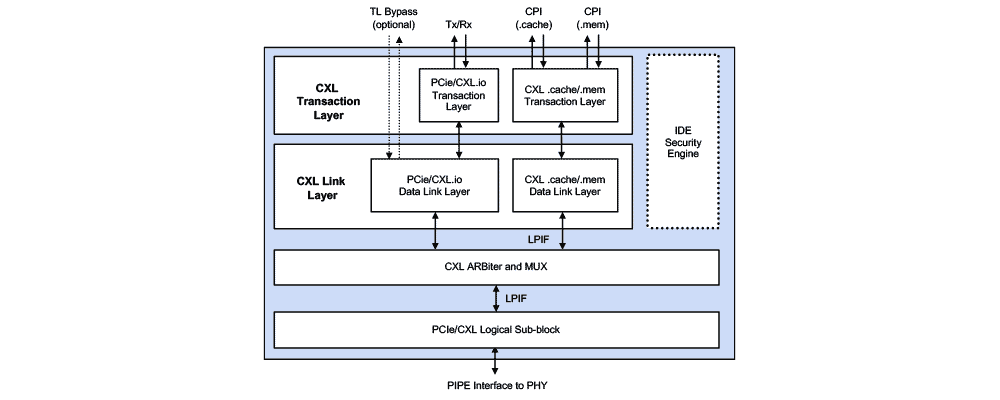
\includegraphics[width=1.2\textwidth]{figs/rambus_cxl31_block.png}
                \caption{Rambus CXL 3.1 Controller Block Diagram}
            \end{figure}
        \end{column}
        \begin{column}{0.48\textwidth}
            \vspace{0.5cm}
            \begin{itemize}
                \item 采用 Rambus 自研 \textbf{PCIe 6.1 PHY IP} 或用户自定义的 \textbf{PIPE 兼容 SerDes} 接口
                \vspace{0.3cm}
                \item PCIe 6.1 \textbf{64\,GT/s}
                \vspace{0.3cm}
                \item IP 核支持\textbf{参数化配置}，可灵活适配不同应用场景
                \vspace{0.3cm}
                \item 提供基于兼容 FPGA SerDes 的\textbf{参考设计}，便于快速 FPGA 原型验证
            \end{itemize}
            \vspace{0.3cm}
            {\footnotesize 参考链接：\href{https://go.rambus.com/l/803123/2023-11-13/47x6dh/803123/170604438955L9Ztqv/CXL_3.1_Controller_Product_Brief.pdf}{Rambus CXL 3.1 Controller Product Brief}}
        \end{column}
    \end{columns}
\end{frame}

% ============================================================
%  澜起 CXL 内存控制器
% ============================================================
\section{澜起 CXL 内存控制器}

\begin{frame}{澜起 CXL 内存控制器}{M88MX6852 —— CXL 3.2 Type 3 内存扩展控制器 (MXC)}
    \begin{columns}[T]


            
        \begin{column}{0.50\textwidth}
            \textbf{关键规格}
            \begin{itemize}
                \item 符合 CXL 1.1 / 2.0 / 3.2，支持 CXL.mem 和 CXL.io
                \item PCIe 6.2 物理层，最高 64 GT/s (x8 通道)
                \item 符合 JEDEC DDR5，最高 DDR5-8000
                \item 支持 UDIMM / RDIMM / On-board DRAM
                \item 内置 CXL 控制器 + DDR 控制器 + RISC-V 微处理器
                \item 丰富的 RAS 功能
                \item 接口：SMBus, I3C/I²C, SPI, JTAG, UART
                \item 封装：1211-ball FCBGA
            \end{itemize}
            \vspace{0.3cm}
            \textbf{典型应用：}内存 AIC 扩展卡、EDSFF 内存模组、\\
            内存数据库、云基础设施、AI/ML 负载

        \end{column}
        \begin{column}{0.48\textwidth}
            \vspace{-3em}
            \begin{figure}
                \centering
                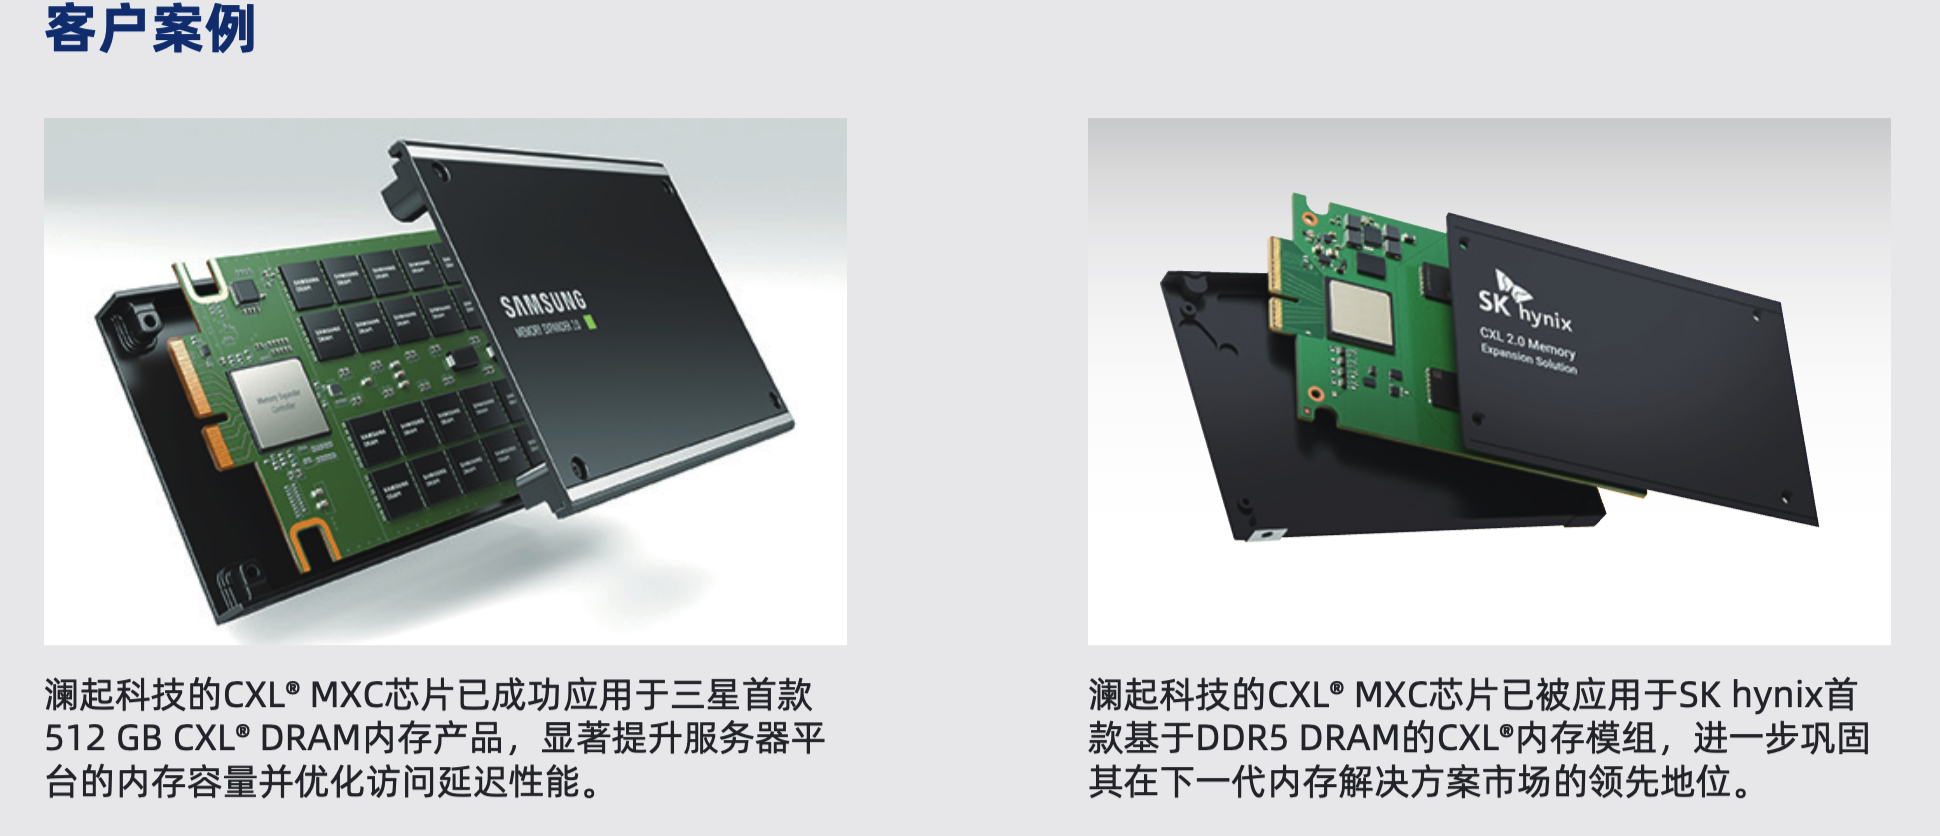
\includegraphics[width=\textwidth]{figs/montage_cases.png}
                \caption{澜起科技 CXL 应用案例}
            \end{figure}
\vspace{-2em}
            \begin{figure}
                \centering
                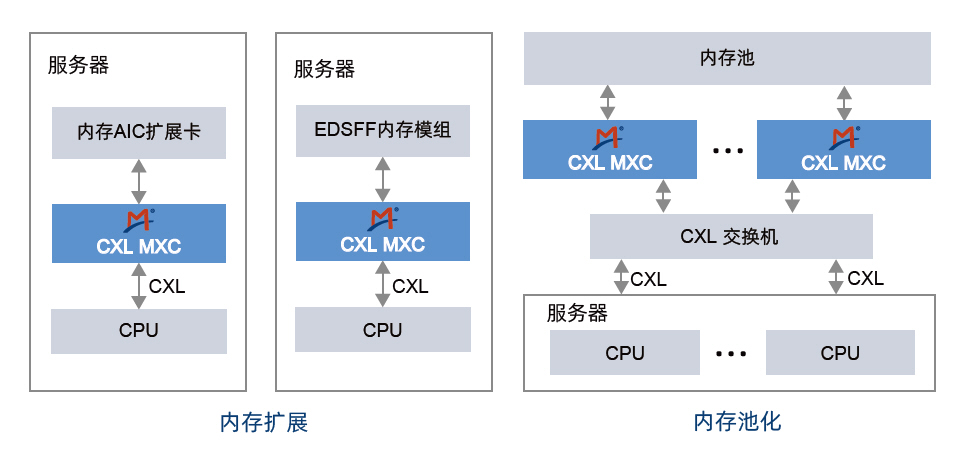
\includegraphics[width=\textwidth]{figs/CXL_Application_CN.jpg}
                \caption{CXL Memory Pooling Architecture}
            \end{figure}
        \end{column}
    \end{columns}
\end{frame}

% ============================================================
%  Asteralab Leo CXL 产品
% ============================================================
\section{Asteralab Leo CXL 产品}

\begin{frame}{Asteralab Leo}{CXL 产品架构}
    \begin{figure}
        \centering
        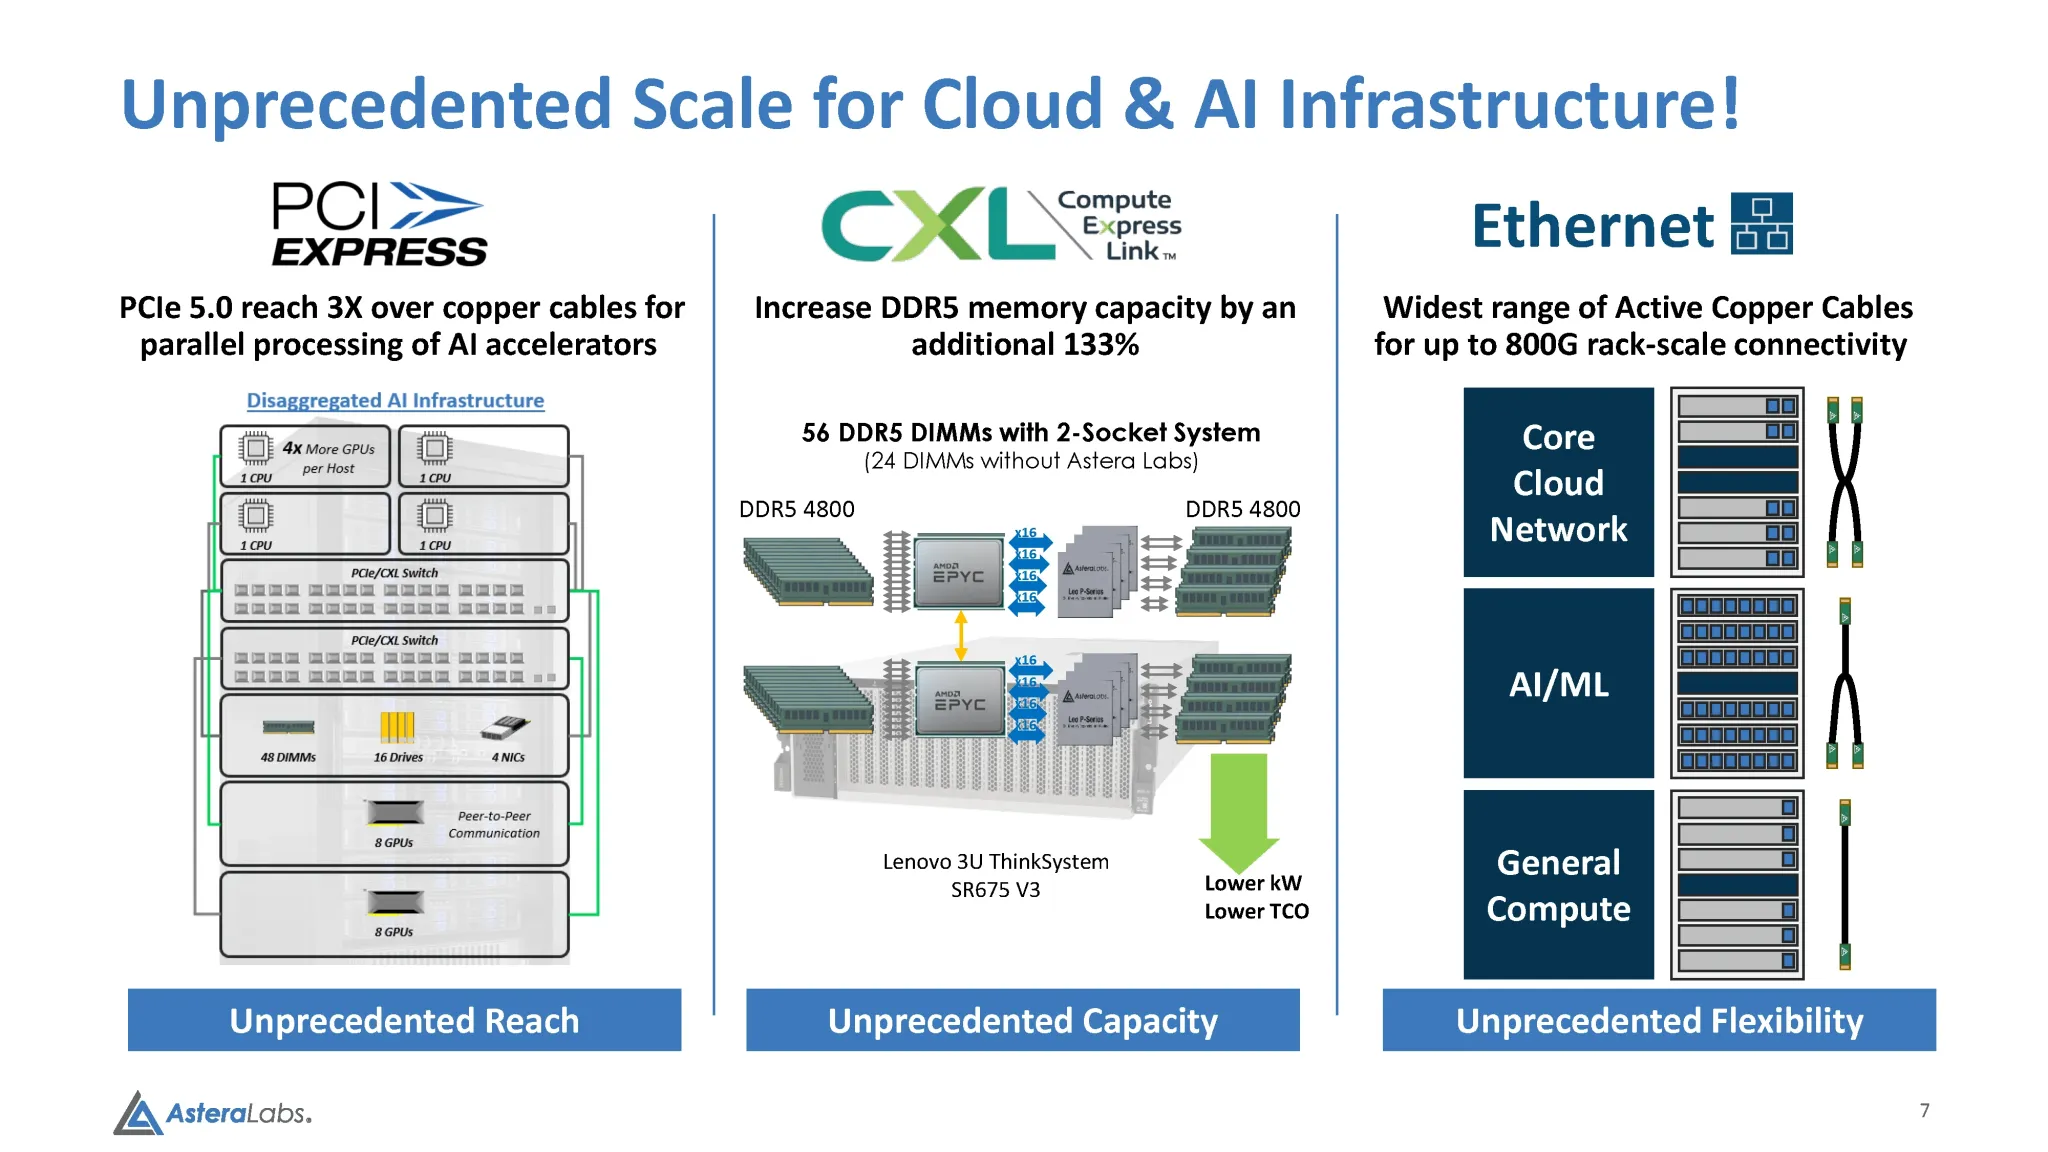
\includegraphics[width=0.85\textwidth]{figs/astera_arch.png}
        \caption{Asteralab Leo CXL 架构图}
    \end{figure}
\end{frame}

% ============================================================
%  Marvell Structera CXL 产品线
% ============================================================
\section{Marvell Structera CXL 产品线}

\begin{frame}{Marvell Structera}{CXL 产品线概览}
    \vspace{-0.3cm}
    \begin{columns}[T]
        \begin{column}{0.48\textwidth}
            \begin{block}{Structera A --- 近存加速器}
                \small
                \textbf{目标：}高带宽应用（DLRM / ML / AI）
                \begin{itemize}
                    \item PCIe 5.0 / CXL 2.0 x16
                    \item 4 通道 DDR5 6400\,MT/s
                    \item 16 \texttimes Arm Neoverse V2 @ 3.2\,GHz
                    \item 带宽 \textbf{200\,GB/s}，容量至 \textbf{4\,TB}
                \end{itemize}
            \end{block}
        \end{column}
        \begin{column}{0.48\textwidth}
            \begin{block}{Structera X --- 内存扩展控制器}
                \small
                \textbf{目标：}高容量应用（内存数据库等）
                \begin{itemize}
                    \item PCIe 5.0 / CXL 2.0 1x16 或 2x8
                    \item X\,2404：4 通道 DDR4 3200\,MT/s，\textbf{12 条 DIMM}
                    \item X\,2504：4 通道 DDR5 6400\,MT/s
                    \item 支持\textbf{双 CPU} 同时访问
                \end{itemize}
            \end{block}
        \end{column}
    \end{columns}

    \begin{block}{共有特性}
        \small
        \begin{itemize}
            \item 业界首款集成 \textbf{Arm Neoverse} 处理器 + \textbf{内联压缩} + \textbf{4 内存通道}
            \item 内联 LZ4 压缩解压缩、AES-XTS 256 位加密、硬件安全模块
            \item 5nm 制程工艺；支持 DDR4 DIMM 回收复用，降低电子垃圾
        \end{itemize}
    \end{block}

    \vspace{0.1cm}
    {\footnotesize 参考链接：\href{https://cn.marvell.com/company/newsroom/marvell-introduces-breakthrough-structera-cxl-product-line-to-address-server-memory-bandwidth-and-capacity-challenges-in-cloud-data-centers.html}{Marvell Structera CXL Product Line Announcement}}
\end{frame}
% ============================================================
%  Marvell Structera 架构图
% ============================================================
\begin{frame}{Marvell Structera}{架构图}
    \begin{figure}
        \centering
        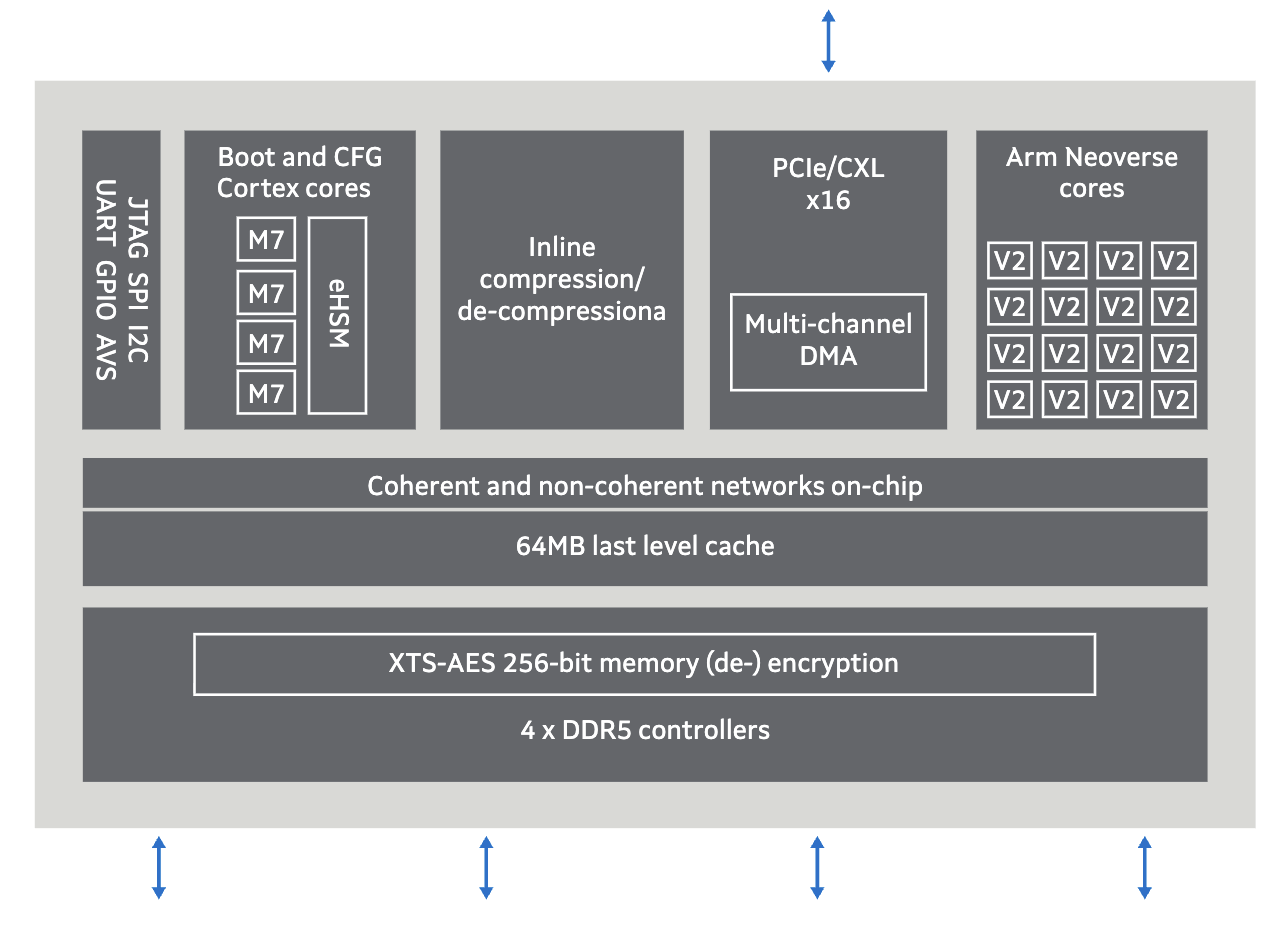
\includegraphics[width=0.6\textwidth]{figs/Marvell_arch.png}
        \caption{Marvell Structera CXL 架构图}
    \end{figure}
\end{frame}
% ============================================================
%  XC50256 CXL 2.0 Switch Chip
% ============================================================
\section{XC50256 CXL 2.0 Switch Chip}

\begin{frame}{XC50256 CXL 2.0 Switch Chip}{世界首款 CXL 2.0 / PCIe Gen 5.0 交换机芯片}
    \begin{columns}[T]
        \begin{column}{0.42\textwidth}
            \begin{figure}
                \centering
                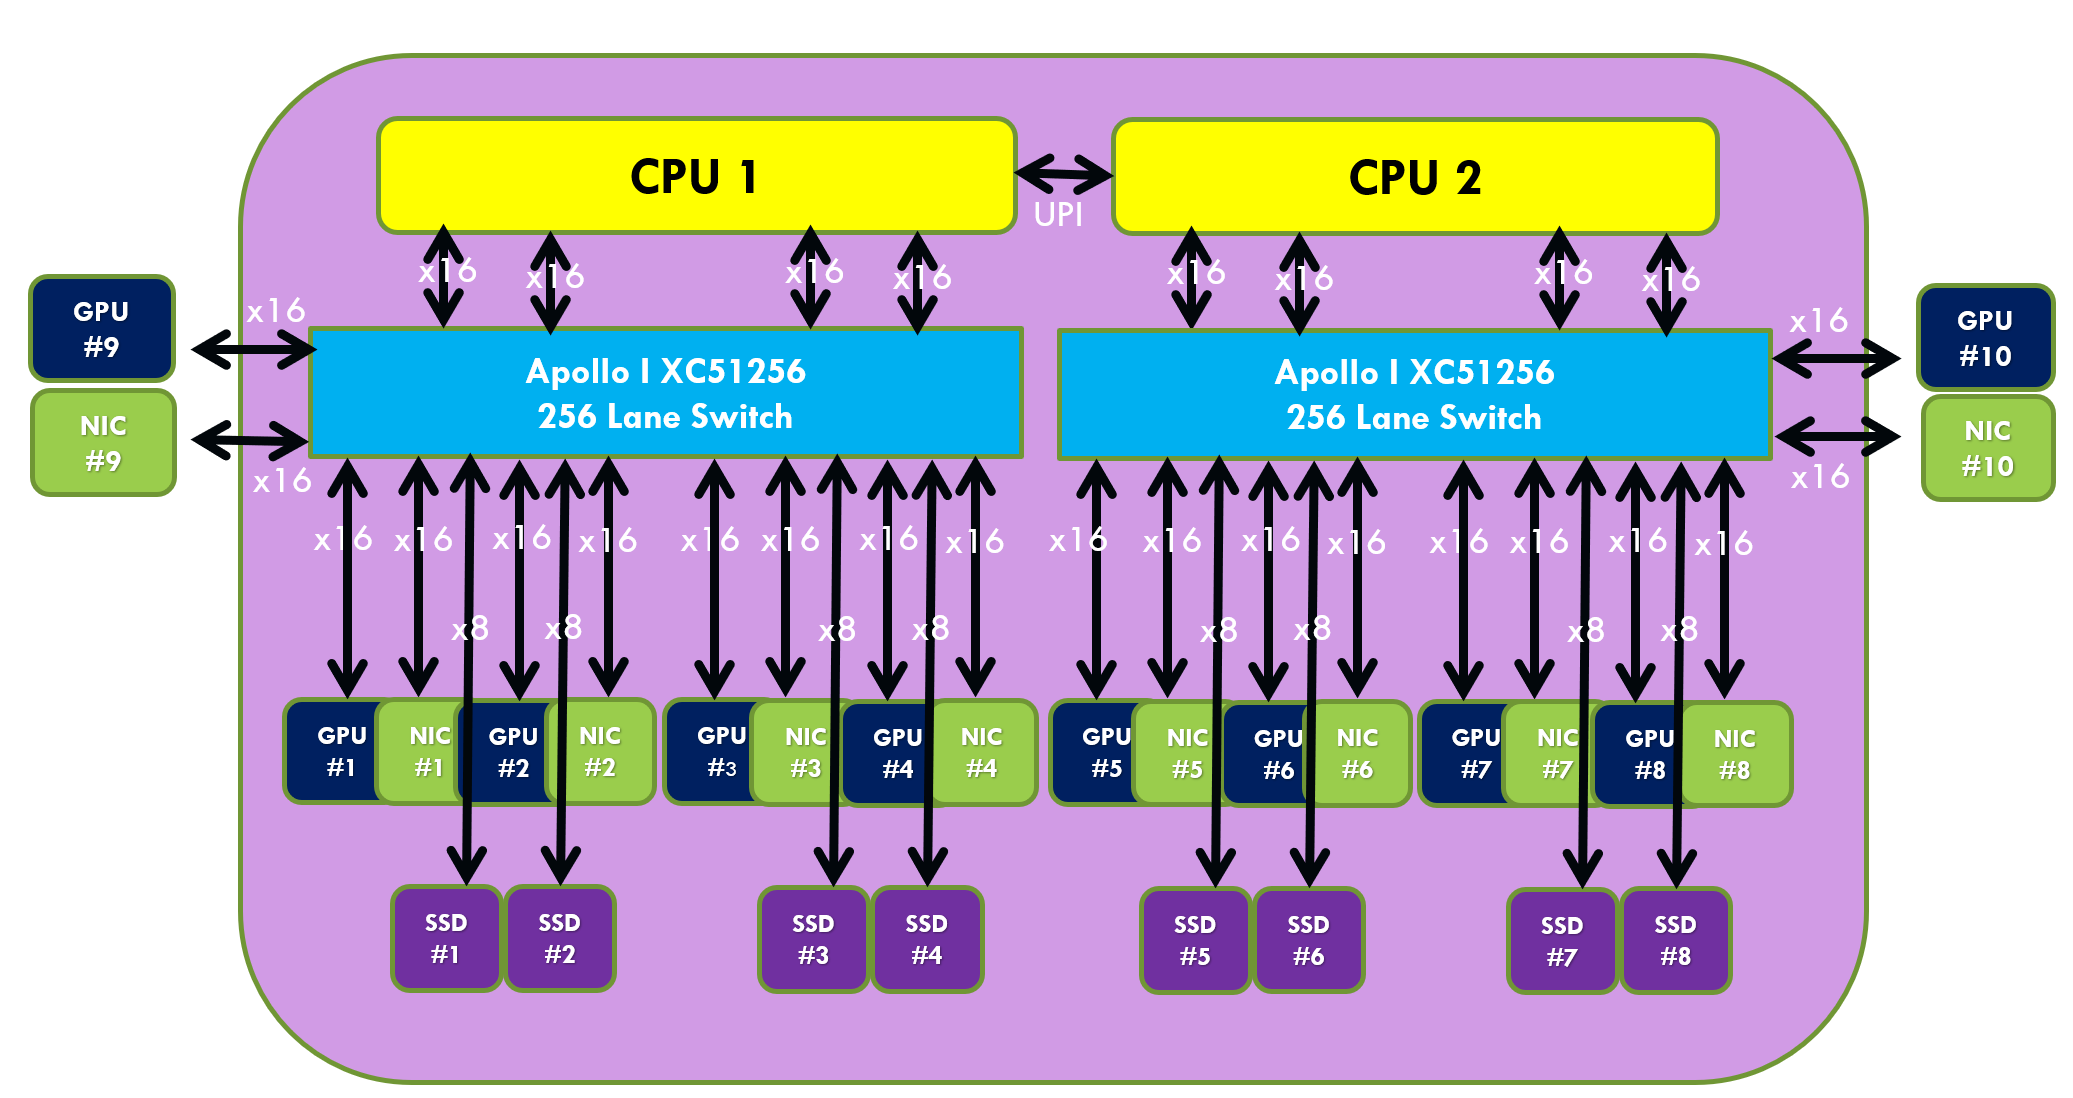
\includegraphics[width=\textwidth]{figs/xconn_km_diagram.png}
                \caption{KM 框图}
            \end{figure}
        \end{column}
        \begin{column}{0.55\textwidth}
            \begin{itemize}
                \item 完全兼容 \textbf{CXL 2.0 / 1.1} 与 \textbf{PCIe Gen 5.0}
                \item 支持 \textbf{CXL.io、CXL.mem、CXL.cache}
                \item CXL Fabric Manager 接口，支持 \textbf{MLD}（Multi-Logical Device）
                \item 多虚拟 CXL 交换机（\textbf{VCS}）
                \item 支持 \textbf{CXL Type 2 / Type 3} 内存设备
                \item 总计 \textbf{32 端口}（含 Bifurcation），\textbf{256 Lane}
                \item 交换容量 \textbf{2,048\,GB/s}
                \item 业内最低端口到端口延迟
                \item 低功耗/端口，减小 PCB 面积，降低 TCO
                \item 完整 RAS 支持：ECC/Parity、DPC、Hot-Plug、Data Poisoning
            \end{itemize}
        \end{column}
    \end{columns}

    \vspace{0.2cm}
    {\footnotesize 参考链接：\href{https://www.xconn-tech.com/products}{XConn Technologies —— Products}}
\end{frame}

% ============================================================
%  XC51256 PCIe Gen 5.0 Switch Chip
% ============================================================
\section{XC51256 PCIe Gen 5.0 Switch Chip}

\begin{frame}{XC51256 PCIe Gen 5.0 Switch Chip}{纯 PCIe 交换机芯片}
    \begin{columns}[T]
        \begin{column}{0.55\textwidth}
            \begin{itemize}
                \item 完全兼容 \textbf{PCIe Gen 5.0} 规范
                \item 业内 \textbf{最低延迟} PCIe Gen 5.0 交换机
                \item 业界 \textbf{最大 Lane 数} PCIe 交换机：\textbf{256 Lane}
                \item x8 / x16 端口 Bifurcation，最多 \textbf{32 端口}
                \item 支持 \textbf{虚拟交换机}、\textbf{非透明桥}（NTB）、\textbf{多主机 IO 共享}
                \item 支持 Hot-Plug、Hot-Add、Hot-Remove、Surprise-Plug
                \item 内嵌逻辑分析仪（\textbf{ELA}）+ Debug GUI 诊断
                \item 接口：I2C、SPI、UART、GPIO、JTAG、SRIS/SRNS
            \end{itemize}
        \end{column}
        \begin{column}{0.42\textwidth}
            \begin{figure}
                \centering
                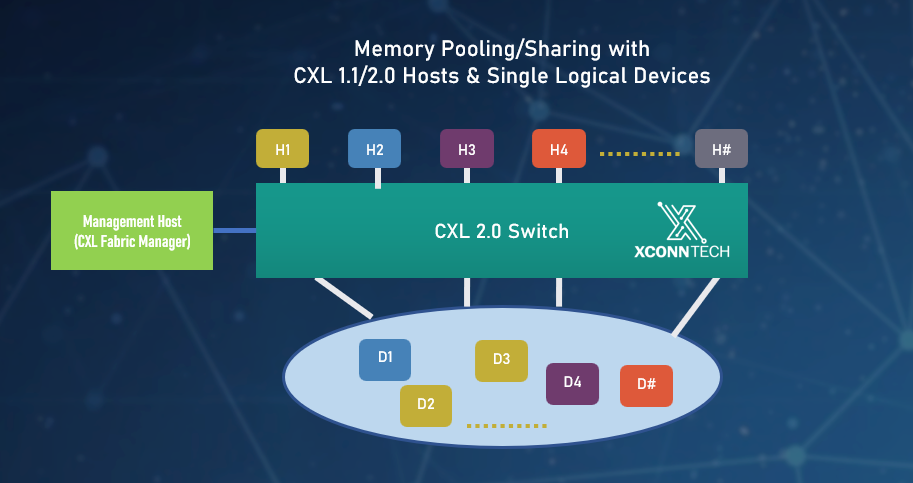
\includegraphics[width=\textwidth]{figs/xconn_chip.png}
                \caption{XC51256 产品图}
            \end{figure}
        \end{column}
    \end{columns}

    \vspace{0.2cm}
    {\footnotesize 参考链接：\href{https://www.xconn-tech.com/products}{XConn Technologies —— Products}}
\end{frame}

\end{document}
